\chapter{Functionality}
\label{chapter:functionality}

The goal of the project ACE is to create a platform independent collaborative text editor. To achieve that goal the editor must satisfy basic text editing functionality as well as collaborative editing functionality.\\

\begin{figure}[H]
\begin{center}
  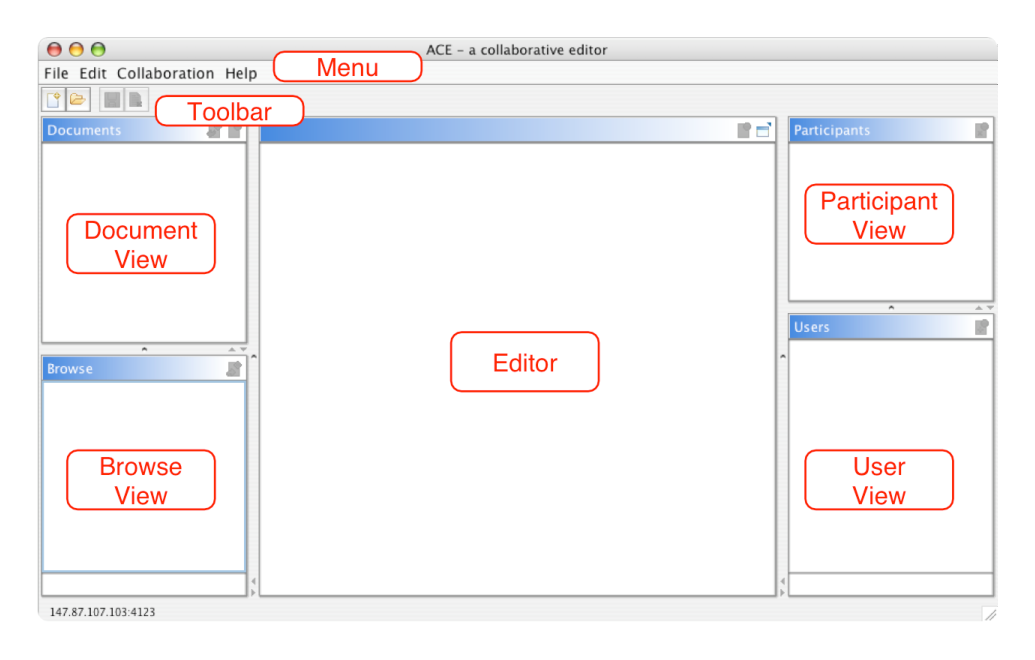
\includegraphics[height=3.1in, width=5.1in]{../images/finalreport/application_ace_overview.eps}
\caption{ACE Overview}
\end{center}
\end{figure}

A basic text editor must provide features like \emph{create new}, \emph{load} and \emph{save} documents. Further it would be user-friendly to have multiple documents open at the same time and switch between them. Operations like cut/copy/paste and undo/redo should not be absent. A more detailed description of the goals can be found in the report \textit{System Requirements: 2.1 Mandatory Goals}. See section \ref{sect:algorithm.undoredo} for a statement why the ACE editor does not support undo/redo.\\

Beside the basic text editor functions, a collaborative text editor must support the \textit{publication} of documents. The published documents should be discovered automatically by all other users running the same collaborative text editor in the same local area network (LAN). This leads to the situation that every user has a list of documents that have been published by other users in the same network. A user can \textit{join} the editing session for such a published document. This means that he starts participating the collaborative editing of the document and he is able to insert, remove or update the content of the document. He also can be \textit{invited} by the owner (publisher) of the published document. To counteract misbehaviour the publisher can \textit{kick} invited users which results in a blacklist entry until they receive a re-invite.

The editor should look very simple and the components should be clearly arranged for the user friendliness. To improve the intuitive handling of the editor, buttons with meaningful images should be positioned at the right and logical place. Also, different colors should be used to highlight the written text and to draw the cursor positions (or selections) in order to make the participants well distinguishable. \\

\begin{figure}[H]
\begin{center}
  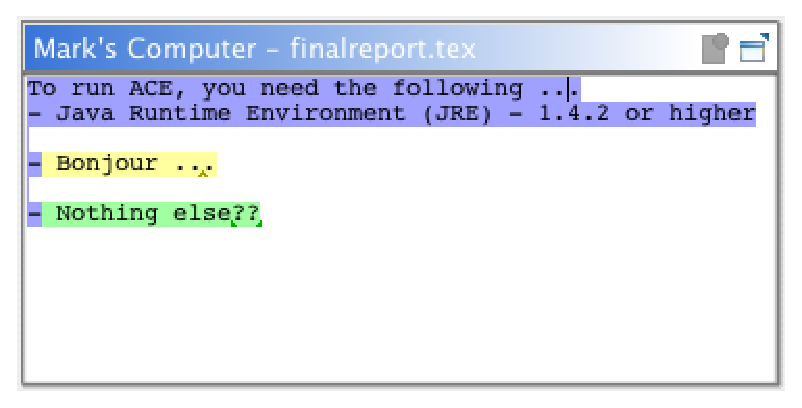
\includegraphics[height=2.5in, width=5.12in]{../images/usermanual/editor_collab_3users.eps}
\caption{Three Users writing in one Document}
\end{center}
\end{figure}

Based on these facts we defined mandatory, optional and non-goals for our diploma work in \textit{System Requirements: Project Goals}. A description of the previous work can be found in \ref{sect:overview.previouswork}.
